\documentclass[tikz,border=16pt]{standalone}
\usepackage{tikz,amsmath,amssymb}
\usetikzlibrary{arrows.meta}

\definecolor{Cd}{HTML}{1f5c9e}   % blue   – diff-equiv   (innermost, strictest)
\definecolor{Co}{HTML}{6a3b90}   % purple – open bisim   (middle)
\definecolor{Ct}{HTML}{2a762a}   % green  – trace equiv  (outermost, weakest)

\begin{document}
	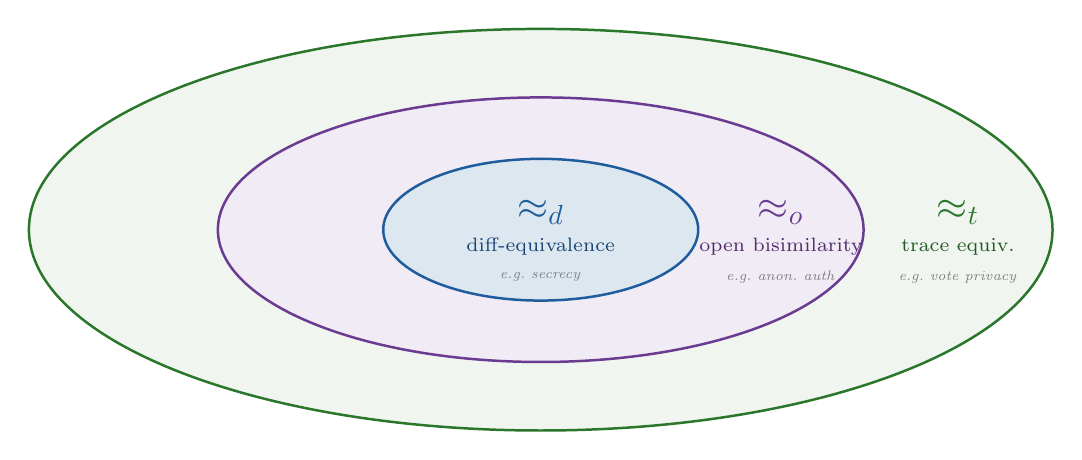
\begin{tikzpicture}
		
		%% formula header
%		\node[font=\normalsize] at (0, 3.35)
%		{$\approx_d\;\subsetneq\;\approx_o\;\subsetneq\;\approx_t$};
		
		%% outermost ellipse — trace equivalence ≈_t
		\draw[Ct, line width=0.9pt, fill=Ct!7]
		(0,0) ellipse (6.50 and 2.55);
		
		%% middle ellipse — open bisimilarity ≈_o
		\draw[Co, line width=0.9pt, fill=Co!10]
		(0,0) ellipse (4.10 and 1.68);
		
		%% innermost ellipse — diff-equivalence ≈_d
		\draw[Cd, line width=0.9pt, fill=Cd!15]
		(0,0) ellipse (2.00 and 0.90);
		
		%% ── labels and scenario tags ──────────────────────────────────────────
		
		%% ≈_d — innermost region (centered)
		\node[font=\Large\bfseries, Cd]          at (0,     0.22) {$\approx_d$};
		\node[font=\scriptsize,      Cd!75!black] at (0,    -0.22) {diff-equivalence};
		\node[font=\tiny,            gray]        at (0,    -0.60) {\textit{e.g.\ secrecy}};
		
		%% ≈_o — right portion of middle ring
		%%   midpoint of right strip: x = (2.00 + 4.10) / 2 = 3.05
		\node[font=\Large\bfseries, Co]          at (3.05,  0.22) {$\approx_o$};
		\node[font=\scriptsize,      Co!75!black] at (3.05, -0.22) {open bisimilarity};
		\node[font=\tiny,            gray]        at (3.05, -0.60) {\textit{e.g.\ anon.\ auth}};
		
		%% ≈_t — right portion of outer ring
		%%   midpoint of right strip: x = (4.10 + 6.50) / 2 = 5.30
		\node[font=\Large\bfseries, Ct]          at (5.30,  0.22) {$\approx_t$};
		\node[font=\scriptsize,      Ct!75!black] at (5.30, -0.22) {trace equiv.};
		\node[font=\tiny,            gray]        at (5.30, -0.60) {\textit{e.g.\ vote privacy}};
		
%		%% ── strictness axis below ellipses ────────────────────────────────────
%		\draw[-{Stealth[scale=0.68]}, gray!55, line width=0.55pt]
%		(0.35, -2.90) -- (5.90, -2.90);
%		\node[font=\tiny, gray, anchor=east] at (0.25, -2.90)
%		{stricter};
%		\node[font=\tiny, gray, anchor=west] at (6.00, -2.90)
%		{weaker};
%		\node[font=\tiny, gray] at (3.15, -3.22)
%		{outward $=$ strictly weaker (more process pairs satisfy the relation)};
		
	\end{tikzpicture}
\end{document}